% En esta sección se deben explicar los riesgos que se materializaron a lo largo del
% proyecto, estuvieran o no previstos al comienzo (más aún si no estaban previstos).
% Por ejemplo, desvíos en las estimaciones que hayan obligado a modificar el alcance,
% interesados con los que esperaban contar que finalmente no estuvieron disponibles, 
% metodologías o tecnologías que no funcionaron como se esperaba, y cuestiones de 
% este estilo.
% Los riesgos no previstos son per se lecciones aprendidas, pero también resulta de 
% interés explicitar qué aspectos del proyecto les dejaron lecciones positivas que 
% hayan servido para el aprendizaje.

\noindent A continuación detallamos los problemas encontrados a lo largo del desarrollo del
Trabajo Profesional. Estos problemas fueron en su mayoría imprevistos que o bien
dificultaron el progreso o bien imposibilitaron el desarrollo de ciertas partes.

\subsection{Deploy de Kubernetes a un ambiente productivo}

\subsection{Shelved game features}

\subsection{Godot Editor}

\subsection{Godot: Optimización de imágenes}

En cierto punto del desarrollo, nos topamos con que cargar nuestro proyecto en el editor de Godot
requería alrededor de 3 GB de memoria RAM y levantar una sola instancia del juego requería también
arriba de 3 GB de memoria principal. En un entorno de desarrollo donde es necesario testear
funcionalidades con por lo menos dos instancias del juego corriendo, esto dificultó e incluso
imposibilitó para algunos integrantes continuar normalmente con el desarrollo. Este requerimiento
de RAM no tenía sentido, ya que la suma del espacio requerido en disco de todos los 
\textit{assets} de nuestro proyecto no superaba los 100 MB.
Luego de investigar más a fondo el problema y entender cómo estábamos cargando los archivos de imágenes,
entendimos mejor cómo las importa Godot y qué implica eso.
Al agregar una imágen al proyecto, Godot genera un archivo con el mismo nombre y extensión 
\textit{.import}, con metadata sobre cómo importar el archivo. Para el caso de las imágenes, 
Godot las importa con un modo de compresión \textbf{Lossless} por defecto. Si bien este modo
tiene la ventaja de que no genera \textit{artifacts} visuales en las imágenes usadas, usa 
considerablemente más memoria VRAM (\textit{Video Random Access Memory}) para almacenar la textura o
imágen importada. La documentación de Godot provee un estimado del espacio que ocupa una sola textura
RGBA8 en la VRAM, dependiendo de las dimensiones de resolución de la imágen. En nuestro caso, como
tenemos una imágen \textit{spritesheet} por cada variante de cada cosmético posible de jugadores,
contábamos con más de 100 imágenes de más de 2048 x 2048 pixeles cada una. 

\begin{figure}[htbp]
    \centering
    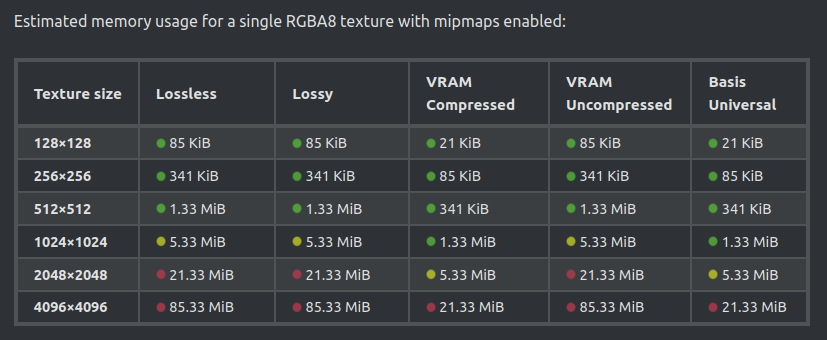
\includegraphics[width=1.0\textwidth]{../assets/godot-docs-images.png}
    \caption{Cuadro comparativo del tamaño que ocupa una imágen en VRAM según la resolución
             de la misma y el modo de compresión utilizado.}
\end{figure}
% https://docs.godotengine.org/en/stable/tutorials/assets_pipeline/importing_images.html

Usando de referencia la tabla de la documentación, y considerando que nuestras imágenes superaban
los 2048 x 2048 pixeles, la memoria en VRAM requerida para nuestro juego tuvo una cota mínima de 
2.24 GB:

\[
\frac{21.33 \, MiB}{imagen} \times 100 \, imagenes = 2.24 \, GB
\]

Para máquinas sin una placa de video dedicada, en lugar de alocar este espacio en VRAM, se aloca
en memoria principal RAM, generando los problemas anteriormente mencionados.
Habiendo hecho este descubrimiento, ahora entendíamos la causa del problema. Para solventarlo,
aplicamos 2 soluciones:

\begin{itemize}
    \item Reducir el tamaño de las imágenes recortándolas, ya que en realidad usamos solo
    una porción de la \textit{spritesheet}.
    \item Cambiar el modo de compresión de los cosméticos para personajes de \textbf{Lossless}
    a \textbf{VRAM Compressed}, para reducir aún más el espacio ocupado de VRAM. Si bien este
    modo de compresión no es recomendado para texturas 2D, especialmente del estilo
    \textit{pixel art} como lo es nuestro juego, al cambiar el modo y volver a correr el juego
    no se notaron defectos ni \textit{artifacts} visuales.
\end{itemize}

Tras haber implementado estos cambios, logramos reducir la memoria requerida por una instancia
del juego a menos de 1 GB.
